% Defense slide 8: sketch of the predicted transfer-matrix spectrum.
% Eigenvalues mu_i in the complex plane: moduli coalescing onto one circle
% while the phases stay separated by pi v x_i / T.
\documentclass[tikz,border=3pt]{standalone}
\usepackage{amsmath,amssymb}
\usetikzlibrary{arrows.meta,calc}

\definecolor{tnbulk}{RGB}{86,196,229}
\definecolor{tnbnd}{RGB}{196,98,22}
\definecolor{tnbox}{RGB}{40,130,70}

\begin{document}
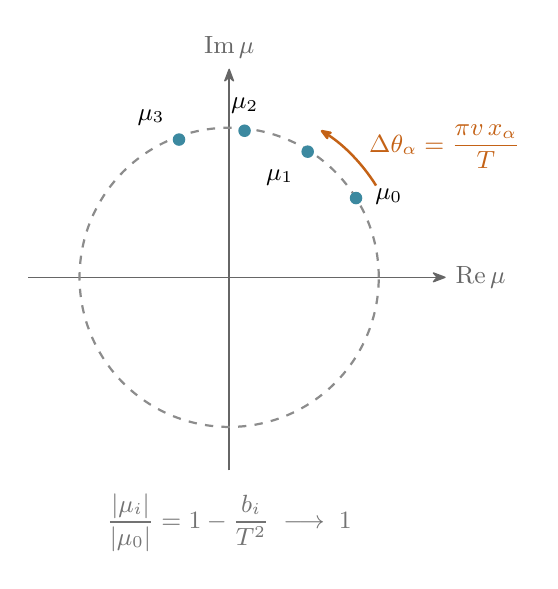
\begin{tikzpicture}[
    >={Stealth[round,length=2.0mm]},
    tag/.style={font=\small},
    pt/.style={circle, fill=tnbulk!70!black, inner sep=1.6pt},
  ]

  \def\R{1.9}

  % axes
  \draw[->, black!60, line width=0.5pt] (-2.55,0) -- (2.75,0) node[right, tag] {$\mathrm{Re}\,\mu$};
  \draw[->, black!60, line width=0.5pt] (0,-2.45) -- (0,2.65) node[above, tag] {$\mathrm{Im}\,\mu$};

  % common-modulus circle
  \draw[black!45, dashed, line width=0.8pt] (0,0) circle (\R);
  % subleading eigenvalues sit slightly INSIDE the circle at finite T
  \node[tag, black!55, anchor=north, align=center] at (0,-2.62)
    {$\dfrac{|\mu_i|}{|\mu_0|} = 1 - \dfrac{b_i}{T^2} \;\longrightarrow\; 1$};

  % eigenvalues: same modulus (nearly), phases separated
  \node[pt] (m0) at (32:{\R}) {};
  \node[pt] (m1) at (58:{\R-0.018}) {};
  \node[pt] (m2) at (84:{\R-0.028}) {};
  \node[pt] (m3) at (110:{\R-0.038}) {};
  \node[tag, anchor=west] at ($(m0)+(0.12,0.02)$) {$\mu_0$};
  \node[tag, anchor=north east] at ($(m1)+(-0.06,-0.10)$) {$\mu_1$};
  \node[tag, anchor=south] at ($(m2)+(0,0.10)$) {$\mu_2$};
  \node[tag, anchor=south east] at ($(m3)+(-0.06,0.06)$) {$\mu_3$};

  % phase gaps
  \draw[->, tnbnd, line width=0.9pt] (32:{\R+0.30}) arc (32:58:{\R+0.30});
  \node[tag, tnbnd, anchor=west] at (45:{\R+0.44})
    {$\Delta\theta_\alpha = \dfrac{\pi v\, x_\alpha}{T}$};

\end{tikzpicture}
\end{document}
